% Dynamic vs Semantic gating flow
\documentclass[tikz,border=5pt]{standalone}
\usepackage{xcolor}
\usepackage{fontspec}
\usetikzlibrary{arrows.meta,shapes.geometric,shadows.blur,positioning}

% Define color scheme
\definecolor{primaryblue}{RGB}{41,128,185}
\definecolor{secondarygreen}{RGB}{39,174,96}
\definecolor{accentorange}{RGB}{230,126,34}
\definecolor{warningred}{RGB}{231,76,60}
\definecolor{lightgray}{RGB}{236,240,241}
\definecolor{darkgray}{RGB}{52,73,94}

\begin{document}
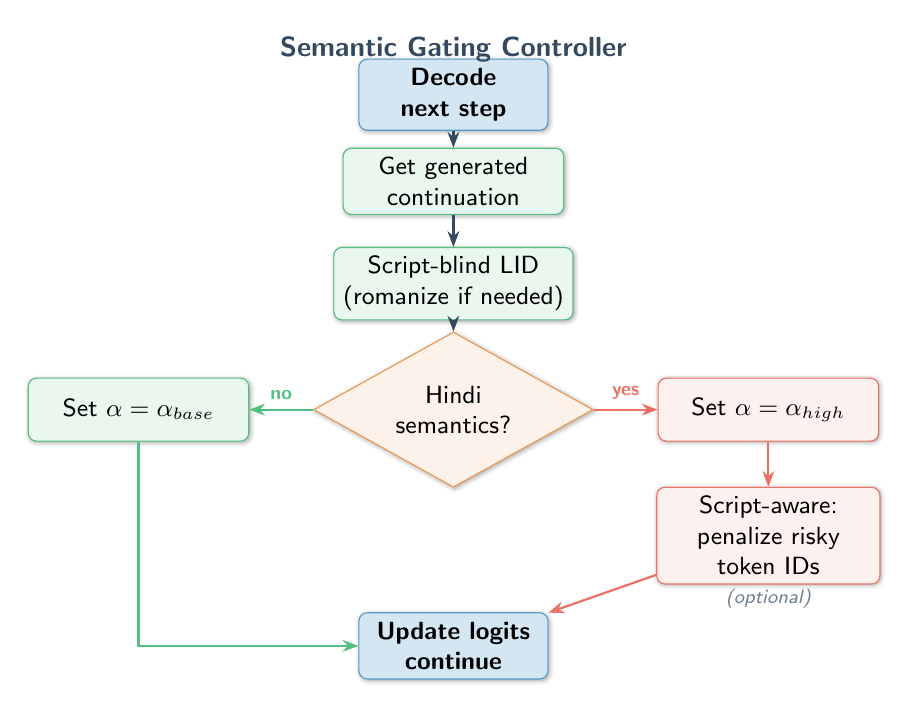
\begin{tikzpicture}[
  node distance=9mm and 14mm,
  startstop/.style={
    draw=primaryblue!80,
    fill=primaryblue!20,
    rounded corners=3pt,
    minimum width=24mm,
    minimum height=8mm,
    align=center,
    font=\sffamily\small\bfseries,
    blur shadow={shadow blur steps=5, shadow xshift=0.5pt, shadow yshift=-0.5pt}
  },
  proc/.style={
    draw=secondarygreen!80,
    fill=secondarygreen!10,
    rounded corners=3pt,
    minimum width=28mm,
    minimum height=8mm,
    align=center,
    font=\sffamily\small,
    blur shadow={shadow blur steps=5, shadow xshift=0.5pt, shadow yshift=-0.5pt}
  },
  decision/.style={
    draw=accentorange!80,
    fill=accentorange!10,
    diamond,
    aspect=1.8,
    align=center,
    font=\sffamily\small,
    blur shadow={shadow blur steps=5, shadow xshift=0.5pt, shadow yshift=-0.5pt}
  },
  action/.style={
    draw=warningred!80,
    fill=warningred!8,
    rounded corners=3pt,
    minimum width=28mm,
    minimum height=8mm,
    align=center,
    font=\sffamily\small,
    blur shadow={shadow blur steps=3, shadow xshift=0.3pt, shadow yshift=-0.3pt}
  },
  line/.style={-{Stealth[length=2mm]}, thick, draw=darkgray},
  yesline/.style={-{Stealth[length=2mm]}, thick, draw=warningred!80},
  noline/.style={-{Stealth[length=2mm]}, thick, draw=secondarygreen!80},
  annot/.style={font=\sffamily\scriptsize\bfseries}
]

% Start
\node[startstop] (start) at (0,0) {Decode\\next step};

% Processing steps
\node[proc] (cont) at (0,-11mm) {Get generated\\continuation};
\node[proc] (lid) at (0,-24mm) {Script-blind LID\\(romanize if needed)};

% Decision point
\node[decision, text width=18mm] (risk) at (0,-40mm) {Hindi\\semantics?};

% Actions based on decision
\node[action] (alphaH) at (40mm,-40mm) {Set $\alpha=\alpha_{\text{high}}$};
\node[proc] (alphaB) at (-40mm,-40mm) {Set $\alpha=\alpha_{\text{base}}$};
\node[action, text width=26mm] (pen) at (40mm,-56mm) {Script-aware:\\penalize risky\\token IDs};

% End
\node[startstop] (end) at (0,-70mm) {Update logits\\continue};

% Draw connections
\draw[line] (start) -- (cont);
\draw[line] (cont) -- (lid);
\draw[line] (lid) -- (risk);

% Decision branches
\draw[yesline] (risk) -- (alphaH) node[midway, above, annot, text=warningred!80] {yes};
\draw[noline] (risk) -- (alphaB) node[midway, above, annot, text=secondarygreen!80] {no};

% Continue from actions
\draw[yesline] (alphaH) -- (pen);
\draw[noline] (alphaB) |- (end);
\draw[yesline] (pen) -- (end);

% Add annotation for script-aware variant
\node[align=center, font=\sffamily\scriptsize\itshape, text=darkgray!70]
  at (40mm,-64mm) {(optional)};

% Add title
\node[anchor=north, font=\sffamily\bfseries, text=darkgray]
  at ($(start.north)+(0,4mm)$) {Semantic Gating Controller};

\end{tikzpicture}
\end{document}
